\documentclass[11pt]{article}

\usepackage[a4paper,margin=1in]{geometry}
\usepackage{amsmath,amssymb,amsthm}
\usepackage{xcolor}
\usepackage[T1]{fontenc}
\usepackage{titlesec}
\usepackage{hyperref}
\usepackage{tikz}
\usetikzlibrary{trees}

% F1R3FLY brand palette
\definecolor{f1rnavy}{HTML}{1A1A2E}
\definecolor{f1rsky}{HTML}{3FA9F5}
\definecolor{f1ryellow}{HTML}{F3D630}
\definecolor{f1rsage}{HTML}{8BB999}

\hypersetup{
  colorlinks=true,
  linkcolor=f1rsky,
  urlcolor=f1rsky,
  citecolor=f1rsage
}

\titleformat{\section}{\Large\bfseries\color{f1rnavy}}{\thesection}{0.6em}{}
\titleformat{\subsection}{\large\bfseries\color{f1rnavy}}{\thesubsection}{0.6em}{}

\renewcommand{\abstractname}{\color{f1rnavy}Brain Candy}

\title{\color{f1rnavy}\textbf{Thompson's Group $F$ as a Theory of Microtonal Retunings}\\[0.3em]
\large\color{f1rsage} A correspondence hiding in plain sight}
\author{\color{f1rnavy}L.~Gregory Meredith\\\small F1R3FLY.io}
\date{\color{f1rnavy}9 April 2026}

\begin{document}
\maketitle

\begin{abstract}
\noindent Richard Thompson's group $F$ --- the group of orientation-preserving piecewise-linear homeomorphisms of $[0,1]$ with dyadic breakpoints and dyadic slopes --- has lived for sixty years inside group theory, logic, and (more recently) Vaughan Jones's program for conformal field theory. We point out that it is also, transparently, the natural group of \emph{hierarchical microtonal retunings of the octave}. Scale degrees are leaves of a binary tree; the tree records the history of how the octave was carved up; an element of $F$ is a pair of such trees with the same number of leaves and acts as a piecewise log-linear retuning sending scale degree to scale degree. The Stein--Brown--Thompson generalisations $F_{n_1,\ldots,n_k}$ are then exactly what one wants for prime-limit just-intonation systems. So far as we can tell, this correspondence has not been written down.
\end{abstract}

\section{The Octave as the Unit Interval}

Fix a reference pitch and parametrise the octave above it logarithmically: $0$ is the reference, $1$ is the octave, and the linear coordinate is exactly cents/$1200$. In this picture, doubling a frequency means moving by $+1$, and a $12$-tone equal-tempered semitone is at $1/12$.

A finite rooted binary tree with $n+1$ leaves now has an obvious meaning: it is a recursive subdivision of the octave into $n+1$ subintervals, where each internal node says ``split this interval into a left half and a right half.'' The leaves are the resulting \emph{scale degrees}, and the tree records the \emph{history} of the carving. Two scales with the same leaf set can have different trees, and that difference is musically meaningful: it encodes which intervals are structurally close to which others.

\begin{center}
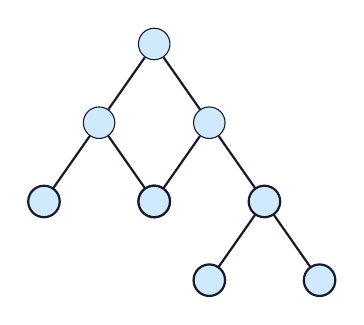
\begin{tikzpicture}[level distance=10mm, sibling distance=14mm,
  every node/.style={circle,draw=f1rnavy,fill=f1rsky!25,inner sep=1.5pt,minimum size=4mm,font=\footnotesize},
  edge from parent/.style={draw=f1rnavy,thick}]
\node {} child {node {} child {node {}} child {node {}}}
        child {node {} child {node {}} child {node {} child {node {}} child {node {}}}};
\end{tikzpicture}
\hspace{1.5em}
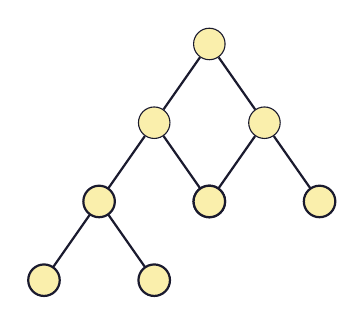
\begin{tikzpicture}[level distance=10mm, sibling distance=14mm,
  every node/.style={circle,draw=f1rnavy,fill=f1ryellow!40,inner sep=1.5pt,minimum size=4mm,font=\footnotesize},
  edge from parent/.style={draw=f1rnavy,thick}]
\node {} child {node {} child {node {} child {node {}} child {node {}}} child {node {}}}
        child {node {} child {node {}} child {node {}}};
\end{tikzpicture}
\end{center}

\section{Elements of $F$ as Retunings}

Recall that an element of $F$ can be presented as a pair $(T_-, T_+)$ of finite rooted binary trees with the same number of leaves; the element acts on $[0,1]$ by ``left tree is the partition you have, right tree is the partition you want,'' linearly interpolating leaf-to-leaf. This is the standard story \cite{CFP}.

Reading the same data in our musical coordinate, an element of $F$ \emph{is} a retuning map between two hierarchically constructed microtonal scales with the same number of notes. It is piecewise log-linear in pitch; on each scale-step interval it is an affine map; the slopes are powers of two, which means the local cent-width of each interval gets doubled, halved, quadrupled, and so on under the retuning. Composition in $F$ is composition of retunings. The identity is a tautological retuning. Inverses go the other way.

Three things deserve emphasis.

\subsection*{The standard generators are a recursion}

The infinite generating set $x_0, x_1, x_2, \ldots$ of $F$ acts as ``caret moves'' progressively deeper down the right spine of the tree. Musically, $x_n$ is the operation: \emph{take the interval at recursion depth $n$ on the upper end of what you have already split, and split it in half.} This is exactly the recipe for octave-reduced harmonic-series approximations and for Bohlen--Pierce-style nested divisions: the asymmetry of $F$ matches the asymmetry of how musicians actually build scales, by repeatedly subdividing the upper remaining interval.

\subsection*{The Brown--Thompson family is the prime-limit hierarchy}

$F$ itself is a 2-limit theory: slopes are powers of $2$, breakpoints are dyadic. Just intonation requires more. The Stein--Brown--Thompson groups $F_{n_1,\ldots,n_k}$ allow slopes that are products of integer powers of the $n_i$ and breakpoints in $\mathbb{Z}[1/n_1,\ldots,1/n_k]$. Choose $\{2,3\}$ and you get the natural group of 3-limit (Pythagorean) retunings; choose $\{2,3,5\}$ and you get 5-limit (just-intonation) retunings; and so on up the prime-limit ladder that microtonalists already use as their organising vocabulary. The Brown--Thompson families and the prime limits are, structurally, the same hierarchy.

\subsection*{Retuning distance is associahedral}

Pairs of binary trees with $n$ leaves are edges in the rotation graph on binary trees, whose vertices are the vertices of the $(n-1)$-associahedron (the Stasheff polytope $K_n$). So the question \emph{what is the minimum number of elementary retunings needed to get from scale $A$ to scale $B$?} is, up to conventions, the diameter problem on the associahedron --- a problem with real machinery and real answers (Sleator--Tarjan--Thurston, Pournin) \cite{STT,Pournin}. ``Distance between scales'' becomes a thing one can compute, not a thing one waves at.

\section{Why This Has Probably Not Been Noticed}

The two communities that hold the pieces of this correspondence have been looking past each other.

The Thompson-groups community, since Vaughan Jones's 2014--2020 program, has been using $F$ and $T$ as discrete approximations to the diffeomorphism group of the circle, in a quest to extract conformal field theories from subfactors \cite{Jones}. The recursive subdivision is interpreted as spacetime, and the reward has been knot and link invariants, irreducible representations, and a long list of operator-algebraic surprises. Pitch never enters.

The mathematical-music-theory community --- the IRCAM/OpenMusic tradition, the Xenharmonic Wiki, the heirs of Erv Wilson and Adriaan Fokker --- has the right musical intuitions (recursive subdivision, prime limits, scale trees), but reaches for cyclic groups $\mathbb{Z}/n\mathbb{Z}$, dihedral groups, and continued fractions / Stern--Brocot mediants. The big infinite group whose elements \emph{are} retunings is sitting one short conceptual step away, but nobody seems to have taken the step.

\section{What a Real Writeup Would Contain}

A proper paper would establish, at minimum: (i) a bijection between hierarchical microtonal scales (with subdivision history) and finite rooted binary trees, made functorial in scale-degree-preserving maps; (ii) the identification of $F$ with the group of 2-limit retunings between such scales, with composition matching musical composition of retunings; (iii) the prime-limit dictionary $\{2,3,\ldots,p_k\} \leftrightarrow F_{2,3,\ldots,p_k}$; (iv) translations of known theorems on $F$ into statements about scales --- for example, the non-amenability question, the structure of the abelianization $F/[F,F] \cong \mathbb{Z}^2$ (which should correspond to two independent ``global stretch'' invariants of a retuning), and the Brown--Geoghegan finiteness results; and (v) the associahedral distance problem as a concrete computational question for microtonal composers.

There is also an obvious bridge to the F1R3FLY world. The rho calculus models concurrent rewrites on hierarchical name structures; the associahedron is the coherence polytope of those rewrites; and the natural group acting on rewrite-histories of a partition is a Thompson-like group. A scale, in this picture, is just a particularly audible rho-process.

\section{Listen to It}

To make the correspondence audible, take the simplest non-trivial example. Two binary trees with five leaves each:

\medskip
\noindent\textbf{Tree A} (right-spine): split $[0,1]$ in half, then split the upper half in half, then split \emph{its} upper half in half, and once more. Leaves at $0, \tfrac12, \tfrac34, \tfrac78, 1$, which on the log-octave are
\[
\text{Scale A} = (0,\ 600,\ 900,\ 1050,\ 1200)\ \text{cents}.
\]
This is the octave-reduced harmonic-series feel: intervals get smaller as you climb.

\medskip
\noindent\textbf{Tree B} (more balanced): split, then split each half. Leaves at $0, \tfrac14, \tfrac12, \tfrac34, 1$, which on the log-octave are
\[
\text{Scale B} = (0,\ 300,\ 600,\ 900,\ 1200)\ \text{cents}.
\]
This is the equal-stepped whole-tone-ish feel.

\medskip

The F-element $(T_A, T_B)$ retunes Scale A to Scale B by piecewise log-linear interpolation, with local slopes $(\tfrac12, \tfrac12, 2, 2)$ --- all powers of two, as required. Composition with its inverse goes the other way. Here is the entire example as a xenpaper score:

\begin{quote}
\ttfamily\small
\{r220Hz\}(1/4)0c 600c 900c 1050c 1200c - 0c 300c 600c 900c 1200c - 1200c 1050c 900c 600c 0c - 1200c 900c 600c 300c 0c
\end{quote}

\noindent Paste it into \href{https://dxinteractive.github.io/xenpaper/}{xenpaper} (or follow \href{https://dxinteractive.github.io/xenpaper/\#\{r220Hz\}(1/4)0c_600c_900c_1050c_1200c_-_0c_300c_600c_900c_1200c_-_1200c_1050c_900c_600c_0c_-_1200c_900c_600c_300c_0c}{this link}) and press play. You will hear: Scale A ascending, Scale B ascending, Scale A descending, Scale B descending. The same five scale degrees, the same melodic shape, retuned through one element of $F$. The ``compression toward the top'' of Scale A versus the even spacing of Scale B is the F-element made audible.

\begin{thebibliography}{9}
\bibitem{CFP} J.~W.~Cannon, W.~J.~Floyd, W.~R.~Parry, \emph{Introductory notes on Richard Thompson's groups}, L'Enseignement Math\'ematique \textbf{42} (1996), 215--256.
\bibitem{STT} D.~D.~Sleator, R.~E.~Tarjan, W.~P.~Thurston, \emph{Rotation distance, triangulations, and hyperbolic geometry}, J.~Amer.~Math.~Soc.~\textbf{1} (1988), 647--681.
\bibitem{Pournin} L.~Pournin, \emph{The diameter of associahedra}, Adv.~Math.~\textbf{259} (2014), 13--42.
\bibitem{Jones} V.~F.~R.~Jones, \emph{Some unitary representations of Thompson's groups $F$ and $T$}, J.~Comb.~Algebra \textbf{1} (2017), 1--44.
\end{thebibliography}

\end{document}
